\subsection[Architektura]{Architektura}
\begin{figure}[H]
    \centering
    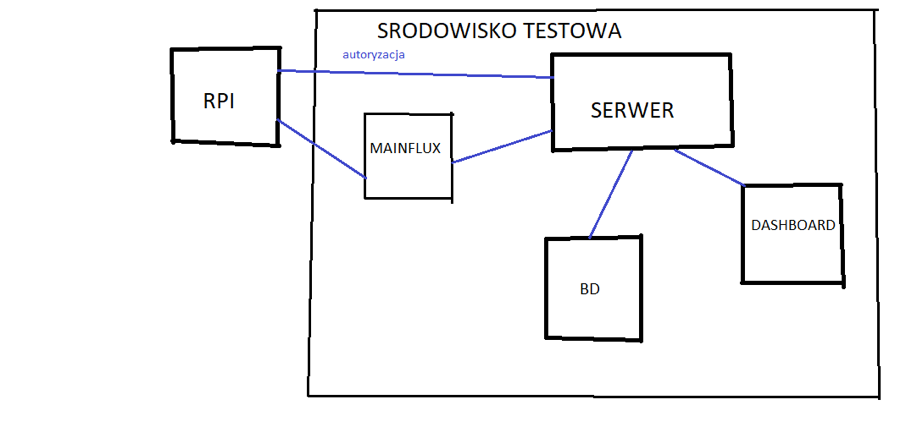
\includegraphics[width=\textwidth]{kp01}
    \caption{Placeholder}
    \label{fig:iotarch}
\end{figure}
SERWER - //jak działa jak jest podzielony //diagram klas dla serwera? 
Serwer ma kilka zadań do spełnienia, pierwszym jest zapewnienie autoryzacji platformy wykonującej. Każda platforma ma swój zewnętrzny identyfikator oraz klucz, w momencie, gdy rpi chce otrzymać swoje dane (tzn. Klucz rzeczy, identyfikator rzeczy oraz 2 przypisane kanały) wysyła HTTP request na serwer z zewnętrznym identyfikatorem oraz kluczem. Serwer po otrzymaniu wiadomości sprawdza czy zewnętrzny identyfikator przesłany przez rpi znajduję się już w bazie danych, jeśli tak to pobiera jego dane oraz zwraca je. W przeciwnym razie serwer dzięki Mainflux-cli loguje się jako administrator, tworzy nową rzecz oraz 2 kanały, po czym przypisuje je do stworzonej rzeczy oraz do rzeczy serwera. Rzecz serwera jest to utworzony obiekt przy starcie środowiska testowego, który ma przypisane do siebie wszystkie kanały. 
Kolejnym zadaniem serwera jest przesyłanie wiadomości z Dashboardu na platforme wykonującą oraz odbieranie wiadomości od rpi. Wysyłanie wiadomości jest stosunkowo łatwe. Wystarczy, że serwer wyśle payloada na odpowiedni kanał, który nasłuchuje w tym samym czasie. Z kolei odbieranie wiadomości jest bardziej skomplikowane, aby odebrać wiadomość serwer musi nasłuchiwać na kanale. Ze względu na to, że wiele platform wykonujących może w tym samym momencie wysyłać wiadomości, środowiko testowe powinno jednocześnie nasłuchiwać na wszystkich kanałach.   Serwer dodaje kanały które znajdują się w bazie danych. Oznacza to, że w momencie gdy nowa platforma wykonująca przechodzi proces autoryzacji, serwer musi automatycznie odświerzyć listę kanałów, które nasłuchują .....???????
Ostatnim zadaniem jest stworzenie rest api, które pozowli na udostępnienie metod "wymaganych przez Dashboard ??". Jednym z celów rest api jest umożliwienie pobrania wiadomości, które platforma wykonująca wysłała na serwer. Pozwala to pentesterowi na przeglądanie wiadomości. Kolejna wystawiona metoda ma za zadanie zwrócić listę aktywnych platform wykonujących. Ta lista znajduje się na serwerze oraz jest uaktualniana co 5 sekund. Uaktualnianie polego na tym, że platforma wykonująca co 2s wysyła wiadomość na serwer z informacją że ciągle jest aktywna jeśli serwer nie otrzyma wiadomości od platformy przez więcej niż 4s aktualne "rpi?? wynik ??" zostaje usunięty. Następną udostępnioną metodą jest wsyłanie payloada na "platformę wykonującą". Serwer pozwala na wysłanie wiadomości do wskazanego rpi lub do wszystkich aktywnych urządzeń.
//rysunek Thing – channel – thing może coś jeszcze o plusch wysyłania na wszystkie platformy